% % % % % % % % % % % % % % % % % % % % % % % % % % % % % % % % % % % % % % % % % % % %
%                                                                                     %
% Short Sectioned Assignment LaTeX Template Version 1.0 (5/5/12)                      %
% This template has been downloaded from: http://www.LaTeXTemplates.com               %
%                                                                                     %
% Original author:  Frits Wenneker (http://www.howtotex.com)                          %
%                                                                                     %
% Modified by: Fco Javier Sueza Rodríguez (fcosueza@disroot.org)                      %
%                                                                                     %
% Changes:                                                                            %
%	    - Custom Chapters, Sections and Subsections (titlesec package)                %
%           - Document type scrbook (oneside)                                         %
%           - Use babel-lang-spanish package and marvosym                             %
%           - Use hyperref, enumitem, tcolorbox and glossaries packages               %
%           - Use Time New Roman (mathptmx), Helvetic and Courier fonts               %
%                                                                                     %
% License: CC BY-NC-SA 3.0 (http://creativecommons.org/licenses/by-nc-sa/3.0/)        %
%                                                                                     %
% % % % % % % % % % % % % % % % % % % % % % % % % % % % % % % % % % % % % % % % % % % %

%-----------------------------------------------%
%	              Packages                  %
%-----------------------------------------------%

\documentclass[paper=a4, fontsize=11pt, oneside]{scrbook}

% ---- Text Input/Output ----- %

\usepackage[T1]{fontenc}
\usepackage[utf8]{inputenc}
\usepackage{mathptmx}
\usepackage[scaled=.92]{helvet}
\usepackage{courier}
\usepackage[indent=12pt]{parskip}

\usepackage{geometry}
\geometry{verbose,tmargin=3cm,bmargin=3cm,lmargin=2.6cm,rmargin=2.6cm}

% ---- Language ----- %

\usepackage[spanish]{babel}
\usepackage{marvosym}

% ---- Another packages ---- %

\usepackage{amsmath,amsfonts,amsthm}
\usepackage{graphics,graphicx}
\usepackage{titlesec}
\usepackage{fancyhdr}
\usepackage{tcolorbox}
\usepackage{hyperref}
\usepackage{enumitem}
\usepackage[automake]{glossaries}

%--------------------------------------------------------------------%
%                      Customizing Document                          %
%--------------------------------------------------------------------%


% ----------- Custom Chapters, Sections and Subsections -------------- %

\titleformat{\chapter}[display]
			{\bfseries\Huge}
			{Tema \ \thechapter} {0.5ex}
			{\vspace{1ex}\centering}

\titleformat{\section}[hang]
			{\bfseries\Large}
			{\thesection}{0.5em}{}

\titleformat{\subsection}[hang]
			{\bfseries\large}
			{\thesubsection}{0.5em}{}

\titleformat{\subsubsection}[hang]
			{\bfseries\large}
			{\thesubsubsection}{0.5em}{}

\hypersetup{
    colorlinks=true,
    linkcolor=black,
    urlcolor=magenta
}

% ------------------- Custom heaaders and footers ------------------- %

\pagestyle{fancyplain}

\fancyhead[]{}
\fancyfoot[L]{}
\fancyfoot[C]{}
\fancyfoot[R]{\thepage}

\renewcommand{\headrulewidth}{0pt} % Remove header underlines
\renewcommand{\footrulewidth}{0pt} % Remove footer underlines

\setlength{\headheight}{13.6pt} % Customize the height of the header

% --------- Numbering equations, figures and tables ----------------- %

\numberwithin{equation}{section} % Number equations within sections
\numberwithin{figure}{section} % Number figures within sections
\numberwithin{table}{section} % Number tables within sections

% ------------------------ New Commands ----------------------------- %

\newcommand{\horrule}[1]{\rule{\linewidth}{#1}} % Create horizontal rule command


%----------------------------------------------------------------------------------------
%	TÍTULO Y DATOS DEL ALUMNO
%----------------------------------------------------------------------------------------

\title{
\normalfont \normalsize
\huge \textbf{Instalación de MySQL y Oracle Database en Windows 10}
}
\author{Francisco Javier Sueza Rodríguez}
\date{\normalsize\today}

%----------------------------------------------------------------------------------------
%                                     DOCUMENTO
%----------------------------------------------------------------------------------------
\begin{document}

\maketitle

\vspace{2ex}

\begin{center}
    \begin{tabular}{l l}
        \textbf{Centro}: & IES Aguadulce \\
        \textbf{Ciclo Formativo}: & Desarrollo Aplicaciones Web (Distancia)\\
        \textbf{Asignatura}: & Bases de Datos\\
        \textbf{Tema}: & Tema 1 - Almacenamiento de la Información \\
    \end{tabular}
\end{center}

\vspace{10ex}

\section{Descripción}
La descripción de los dos apartados de los que consta esta actividad es la siguiente:

\begin{itemize}
    \item \textbf{Apartado 1}: Instalación de MySQL Community Server 8.0.30 (que incluye MySQL Server y MySQL Workbench)
    \begin{enumerate}
        \item Descarga en tu ordenador el producto MySQL Community Server 8.0.30 para el S.O que tengas instalado. Puedes encontrarlo en la página oficial de \href{https://dev.mysql.com/downloads/mysql/}{MySQL}.
        \item Inicia, desde la ubicación donde lo hayas descargado, el instalador del producto y completa la instalación.
        \item Ejecuta MySQL Workbench  y accede a su página principal sin lleguar a establecer ninguna conexión.
        \item Establece una conexión con el usuario administrador 'root' y utiliza la contraseña que hayas establecido durante el proceso de instalación.
        \item Una vez que te hayas autenticado con el usuario administrador, crea un usuario nuevo estableciendo el nombre de usuario y la contraseña. (Los demás valores de la configuración: roles, privilegios,....déjalos por defecto).
        \item Establece una conexión con el nuevo usuario.
    \end{enumerate}
    \item \textbf{Apartado 2}: Instalación de Oracle Database Express Edition 11g Release 2
    \begin{enumerate}
        \item Descarga en tu ordenador el producto Oracle Database Express Edition 11g R2 que puedes encontrarlo en la página oficial de \href{https://www.oracle.com/database/technologies/xe-prior-release-downloads.html}{Oracle} o bien en estos enlaces:
        \begin{itemize}
            \item \href{https://www.filehorse.com/es/descargar-oracle-database-express/27799/}{Oracle Express Edition 11g Release (32 bits) Windows}
            \item \href{https://www.filehorse.com/es/descargar-oracle-database-express/27798/}{Oracle Express Edition 11g Release (64 bits) Windows}
            \item \href{https://www.tuinformaticafacil.com/descargas-gratis/bases-de-datos/herramientas-oracle/oracle-database-express-edition-11g-r2-para-linux-x64}{Oracle Express Edition 11g Release (64 bits) Linux}
        \end{itemize}
    \item Inicia, desde la ubicación donde lo hayas descargado, el instalador del producto y completa la instalación.
    \item Ejecuta Oracle Database Express Edition 11g R2 y accede a su página principal a través del navegador web que desees.
    \item Inicia sesión con el usuario administrador estándar de Oracle Express y utiliza la contraseña que hayas establecido durante el proceso de instalación.
    \item Una vez que te hayas autenticado con el usuario administrador, crea un espacio de trabajo con su usuario correspondiente.
    \item Entra en el espacio de trabajo con el usuario autenticado.
    \end{enumerate}
\end{itemize}

\section{Instalación de MySQL}
MySQL es un SGBD (Sistema Gestor de Bases de Datos) realizado bajo licencia dual (GPL/Comercial) por Oracle Corpotation y es considerada como la base de datos de código abierto más popular del mundo y una de las más populares junto a Oracle y Microsoft SQL Server, sobre todo para entornos de desarrollo web. \cite{mysql}.

En esta sección, vamos a realizar la instalación y configuración de su versión libre, \textbf{MySQL Community Server 8.0.30}, en el sistema operativo Windows 10, creando posteriormente un nuevo usuario y realizando una conexión con este. Para ello, vamos a seguir los siguientes pasos:

\begin{enumerate}
    \item En primer lugar, vamos a descargar el instalador oficial de MySQL para Windows 10. Lo podemos encontrar en la \href{https://dev.mysql.com/downloads/installer/}{web oficial de MySQL}. En la imagen de abajo, se muestra la página de descarga, resaltando la versión que deberemos descargar.

    \begin{figure}[ht]
        \centering
        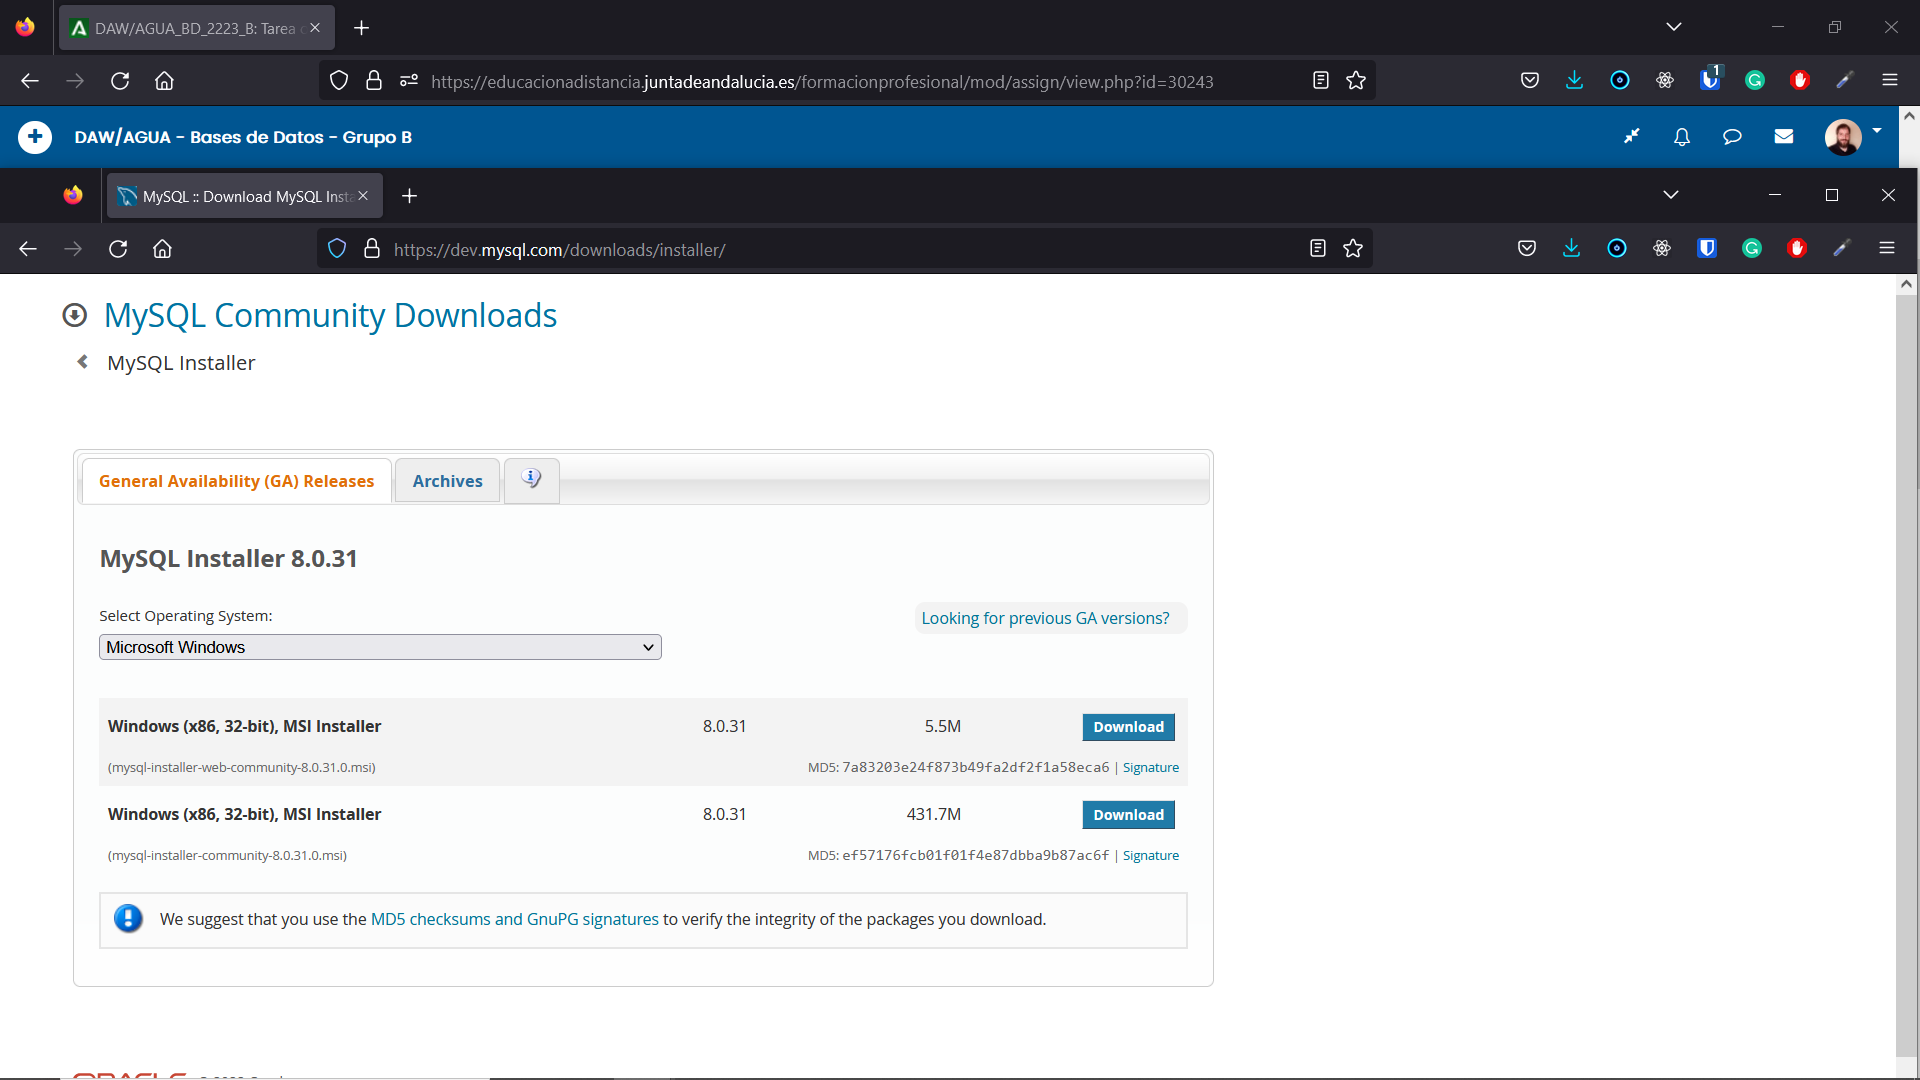
\includegraphics[scale=0.35]{descarga-mysql.png}
        \caption{Página de descarga del instalador de MySQL}
    \end{figure}
\end{enumerate}


% Bibliography

\newpage
\bibliography{citas}
\bibliographystyle{unsrt}

\end{document}